% $Id: template.tex 11 2007-04-03 22:25:53Z jpeltier $

\documentclass{vgtc}                          % final (conference style)
%\documentclass[review]{vgtc}                 % review
%\documentclass[widereview]{vgtc}             % wide-spaced review
%\documentclass[preprint]{vgtc}               % preprint
%\documentclass[electronic]{vgtc}             % electronic version


%% Uncomment one of the lines above depending on where your paper is
%% in the conference process. ``review'' and ``widereview'' are for review
%% submission, ``preprint'' is for pre-publication, and the final version
%% doesn't use a specific qualifier. Further, ``electronic'' includes
%% hyperreferences for more convenient online viewing.

%% Please use one of the ``review'' options in combination with the
%% assigned online id (see below) ONLY if your paper uses a double blind
%% review process. Some conferences, like IEEE Vis and InfoVis, have NOT
%% in the past.

%% Figures should be in CMYK or Grey scale format, otherwise, colour 
%% shifting may occur during the printing process.

%% These few lines make a distinction between latex and pdflatex calls and they
%% bring in essential packages for graphics and font handling.
%% Note that due to the \DeclareGraphicsExtensions{} call it is no longer necessary
%% to provide the the path and extension of a graphics file:
%% \includegraphics{diamondrule} is completely sufficient.
%%
\ifpdf%                                % if we use pdflatex
  \pdfoutput=1\relax                   % create PDFs from pdfLaTeX
  \pdfcompresslevel=9                  % PDF Compression
  \pdfoptionpdfminorversion=7          % create PDF 1.7
  \ExecuteOptions{pdftex}
  \usepackage{graphicx}                % allow us to embed graphics files
  \DeclareGraphicsExtensions{.pdf,.png,.jpg,.jpeg} % for pdflatex we expect .pdf, .png, or .jpg files
\else%                                 % else we use pure latex
  \ExecuteOptions{dvips}
  \usepackage{graphicx}                % allow us to embed graphics files
  \DeclareGraphicsExtensions{.eps}     % for pure latex we expect eps files
\fi%

%% it is recomended to use ``\autoref{sec:bla}'' instead of ``Fig.~\ref{sec:bla}''
\graphicspath{{figures/}{pictures/}{images/}{./}} % where to search for the images

\usepackage{microtype}                 % use micro-typography (slightly more compact, better to read)
\PassOptionsToPackage{warn}{textcomp}  % to address font issues with \textrightarrow
\usepackage{textcomp}                  % use better special symbols
\usepackage{mathptmx}                  % use matching math font
\usepackage{times}                     % we use Times as the main font
\renewcommand*\ttdefault{txtt}         % a nicer typewriter font
\usepackage{cite}                      % needed to automatically sort the references
\usepackage{tabu}                      % only used for the table example
\usepackage{booktabs}                  % only used for the table example
%% We encourage the use of mathptmx for consistent usage of times font
%% throughout the proceedings. However, if you encounter conflicts
%% with other math-related packages, you may want to disable it.


%% If you are submitting a paper to a conference for review with a double
%% blind reviewing process, please replace the value ``0'' below with your
%% OnlineID. Otherwise, you may safely leave it at ``0''.
\onlineid{0}

%% declare the category of your paper, only shown in review mode
\vgtccategory{Research}

%% allow for this line if you want the electronic option to work properly
\vgtcinsertpkg

%% In preprint mode you may define your own headline.
%\preprinttext{To appear in an IEEE VGTC sponsored conference.}

%% Paper title.

\title{The accessibility of cities in metropolitan France}

%% This is how authors are specified in the conference style

%% Author and Affiliation (single author).
%%\author{Roy G. Biv\thanks{e-mail: roy.g.biv@aol.com}}
%%\affiliation{\scriptsize Allied Widgets Research}

%% Author and Affiliation (multiple authors with single affiliations).
%%\author{Roy G. Biv\thanks{e-mail: roy.g.biv@aol.com} %
%%\and Ed Grimley\thanks{e-mail:ed.grimley@aol.com} %
%%\and Martha Stewart\thanks{e-mail:martha.stewart@marthastewart.com}}
%%\affiliation{\scriptsize Martha Stewart Enterprises \\ Microsoft Research}

%% Author and Affiliation (multiple authors with multiple affiliations)
\author{Elia-Swarth \thanks{email:}\\ %
       %
\and Xian\thanks{e-mail: xian@aol.com}\\ %
      %
\and Aujogue Jean-baptiste\thanks{e-mail: jb.aujogue@gmail.com}} %
     
%% A teaser figure can be included as follows, but is not recommended since
%% the space is now taken up by a full width abstract.
%\teaser{
%  \includegraphics[width=1.5in]{sample.eps}
%  \caption{Lookit! Lookit!}
%}

%% Abstract section.
%\abstract{} % end of abstract

%% ACM Computing Classification System (CCS). 
%% See <http://www.acm.org/about/class> for details.
%% We recommend the 2012 system <http://www.acm.org/about/class/class/2012>
%% For the 2012 system use the ``\CCScatTwelve'' which command takes four arguments.
%% The 1998 system <http://www.acm.org/about/class/class/2012> is still possible
%% For the 1998 system use the ``\CCScat'' which command takes four arguments.
%% In both cases the last two arguments (1998) or last three (2012) can be empty.

\CCScatlist{
  \CCScatTwelve{Accessibility}{Travel times}{Visualization}{}
}

%\CCScatlist{
  %\CCScat{H.5.2}{User Interfaces}{User Interfaces}{Graphical user interfaces (GUI)}{};
  %\CCScat{H.5.m}{Information Interfaces and Presentation}{Miscellaneous}{}{}
%}

%% Copyright space is enabled by default as required by guidelines.
%% It is disabled by the 'review' option or via the following command:
% \nocopyrightspace

%%%%%%%%%%%%%%%%%%%%%%%%%%%%%%%%%%%%%%%%%%%%%%%%%%%%%%%%%%%%%%%%
%%%%%%%%%%%%%%%%%%%%%% START OF THE PAPER %%%%%%%%%%%%%%%%%%%%%%
%%%%%%%%%%%%%%%%%%%%%%%%%%%%%%%%%%%%%%%%%%%%%%%%%%%%%%%%%%%%%%%%%

\begin{document}

%% The ``\maketitle'' command must be the first command after the
%% ``\begin{document}'' command. It prepares and prints the title block.

%% the only exception to this rule is the \firstsection command
\firstsection{Introduction}

\vspace{0.2cm}

\maketitle
There is an undoubted concentration phenomenon of population and activity towards certain nerve centers, that constitute our cities and urban areas. The accessibility of a city has an accelerating effect on this phenomenon, accompanying at a deep level the transformation of the city's demography, activity and culture \cite{RePEc:mtp:titles:0262561476}. In this sense, accessibility has even become of strategical importance in order to drain investments, skills and tourism.

%\vspace{0.2cm}

 In this work, we aim at proposing a solution to visualize such an accessibility factor for a city. Here the accessibility factor of a city is computed in a rather trivial, yet natural way: It is expressed as the travel time towards this city, averaged out over the territory of metropolitan France. There certainly exist more sophisticated and realistic ways to define such an accessibility factor, and we slightly discuss this as a possible perspective of work in the ending section.

%\vspace{0.2cm}

After a brief presentation on existing studies of the socio-economic impact of city accessibility, we shall provide a detailed presentation of our visualization solution. A chart-based presentation will be the main object of this visualization. Indeed, this option provides an instantaneous reading of the relevant information, and also provides a realistic distribution of cities among the territory, thus giving the possibility to easily notice differences between travel times with actual geographical distances.

%\vspace{0.2cm}

The visualization should be divided into two parts: A first part should carry in a synthetic way the global information of accessibility of cities across the territory. Then a second part should provide, in an interactive fashion, details on how easily a particular city may be reached, depending on the starting location. We are interested here in two main travel options, namely car and train. The visualization should therefore display accessibility with respect to both of these transportation options.

%\vspace{0.2cm}

 Another quantity that dramatically impacts the traffic fluidity, and thus the accessibility of a city, it that of the period of time within a year. We therefore aim at developing the possibility for the user to switch between seasons in order to have an demonstration of this effect. The time granularity should obviously be refined to get a better description of the impact of time on real-time accessibility of a city, and we leave this aspect for discussion in the concluding paragraph. 


\vspace{0.2cm}
\section{Related work}

\vspace{0.1cm}

%\subsection{Historique de l'étude de l'accessibilité au sein d'un territoire}

%\vspace{0.3cm}
\subsection{Socio-economic impact of accessibility}

\vspace{0.2cm}

Pour une étude de l'impact de l'efficacité du réseaux intra-urbain sur le marché de l'emploi au seins des grandes villes de France on peut consulter \cite{}.

In the everyday life accessibility may easily be observed: It indeed is the cause of direct and indirect creation of jobs, a raise in corporation productivity, enforce new partnerships, facilitate exchanges, and reduces transport costs and its environmental impact.



Dans ce travail, on souhaite montrer le degré d'accessibilité des principales villes de France metropolotaine. 
% Concentration de l'activité dans les centres névralgiques de réseaux. Une répartition uniforme des voies de transport au sein d'un territoire permet la formation de zones économiquement autonomes.

Une mauvaise accessibilité peut etre une raison suffisante pour un bachelier de ne pas effectuer ses études dans ladite région



L'étude des phénomenes de concentration de population (et donc de la puissance economique) en certains poles prend évidement en compte l'accessibilité de ces poles comme facteur d'accélération de cette concentration et l'excusivité de ces poles 

\subsection{Existing visualization methods and case-studies}

\vspace{0.2cm}

De nombreuses visualisation de l'état du traffic à grande échelle (et à petite échelle) sont disponibles. La figure 1 ci-apres montre une visualisation des temps de trajet vers Paris, suporposant ces temps sur une période de 200 ans, qui remonte à 130 ans en arriere ! pour une discussion à ce propos on pourra consulter \cite{schoedon2016interactive}.  Pour une présentation vulgarisée bien plus récente sur l'évolution des temps de trajet en train on pourra voir \cite{LeMonde1}.



\begin{figure}[h]
 \centering % avoid the use of \begin{center}...\end{center} and use \centering instead (more compact)
 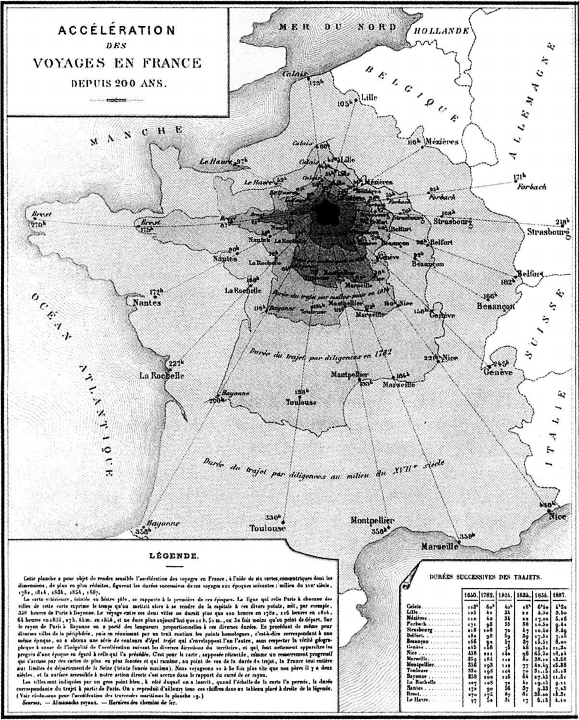
\includegraphics[scale=1, width=\columnwidth]{Fig-15-Anamorphic-map-Acceleration-of-Travel-in-France-over-200-Years-Acceleration}
 \caption{\textit{Acc\'el\'eration des voyages en France depuis 200 ans}, from \cite{Cheysson} }
 \label{fig:sample}
\end{figure}




La quantité d'articles traitant de l'impact des réseaux de transport sur la société est immense. Des revues entieres sont dédiées à ce sujet. Pour une lecture de certains aspects de l'impact de la géométrie du réseau de chemain de fer on pourra par exemple lire \cite{cao2017investigating} et les references mentionnées.


\section{Presentation of our visualization}

\vspace{0.1cm}

\subsection{Data acquisition}

\vspace{0.2cm}

The data of traveling time between two geographical points on the globe are extremely rich and can be obtained e.g. through the Google \textit{Distance Matrix} API \cite{APIGoogle},
by sending a request in form of a URL, in which information such as city of departure, city of arrival, means of transportation (train or automobile) and traveling date should be specified.  
  
%\vspace{0.2cm}

For the reason that, as users of the free version of this service, we are only allowed to initiate requests with a very limited numbers of cities of departure and arrival (10 at a time), it is necessary to automatize the procedure of data acquisition. In order to do this we've written a program in Python which, based on a series of French cities numbered after their population size, takes as parameters a range of departure and arrival cities, the transport means and date that we need, and returns the URL of the corresponding request in the right format. Putting the URL in a web browser returns the desired data, in the form of a .json file, which is then fed to another Python program, the latter returning the traveling time between any two cities included in the request, for the selected transportation means and date.  

%\vspace{0.2cm}

The number of journeys to be treated dramatically increases as more cities and dates are considered, and storing the entire amount of traveling times between all places that one can name all over the country is simply out of reach. However, we still would like to enable the user to add a desired city upon request: This would consist in providing a field, into which the user may enter a place of his choice in order to obtain its accessibility.



\subsection{Visualization structure}

The visualization of cities accessibility starts in the first place with a synthetic view: a topographic map of France, where "mountains" represent cities
that are easier to access in general and valleys the ones who have a lower mean accessibility.  
  
The main part of the visualization takes the form of a national map as well. However, here, the user is asked to position his cursor over a city.
This action will trigger off a coloration of the maps, whether in gradually changing gray or in contour blocks, as being shown in the figure, where
the shade of the color represents the travelling time from other places of France to this city (or the other way round from this city to other places).
The advantages to use a colored map in our visualization are here very clear: one can not only rapidly grasp the accessiblity of other places in France
with respect to this city, but the comparison of the distances in terms of travelling time to the geographical ones is also immediate.
It is noteworthy as well that we offer the user two options in the visualization: he could switch between railway and automobile as transportation means and between
summer and winter as the season that the journey should take place, for the reason that depending on the month of a year, the SNCF timtable and tha road condition of the highways could also vary.
Plus, we give the user the possiblity to select both of the tranportation means. In that case, the map will be displayed with two colors,
each of them representing respectively train or car, indicating the quicker way to get to a place. Again, we find such representation with a colored map very attractive, in the way that
it could bring immediately the competitivity of both transportations means to light.





\vspace{0.2cm}

La visualisation de l'accessibilité de chaque ville passe d'abord par une vue synthétique: Une seule carte du territoire, couverte par une surface ondulante, dont les pics correspondent aux zones les plus accessibles et les creux aux zones les moins accessibles. 

Le corps de la visualisation se présente également sous forme d'une carte du territoire, mais ou l'utilisateur est demandé de pointer une ville. Cette action déclenche une coloration de la carte, en nuances de gris ou par paliers de couleurs, qui permet de représenter le temps de trajet depuis n'importe quel point jusqu'à cette ville (ou inversement, depuis cette ville jusqu'à n'importe quel point de la carte). Les avantages d'une représentation par carte par rapport à d'autres solutions de visualisation sont multiples: On saisit en un instant la répartition des zones les plus accessibles depuis cette ville, et la comparaison avec la distance géographique réelle est immédiate. Dans cette visualisation deux options seront disponibles: Celle de choisir entre mode de transport (voiture et train), et celle de choisir la saison (été ou hiver). 


\begin{figure}[tb]
 \centering % avoid the use of \begin{center}...\end{center} and use \centering instead (more compact)
 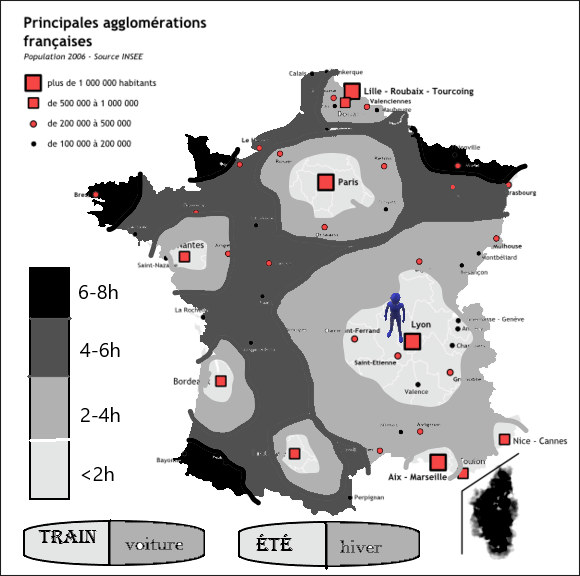
\includegraphics[scale=1, width=\columnwidth]{carte-france23.png}
 \caption{A visualization of traveling times towards the city of Lyon.}
 \label{fig:sample}
\end{figure}

%\begin{center}
%INSERT VIZU HERE\\
%champs scalaires / carte de topographie contours ?
%\end{center}


Nous mettons également à disponibilité la possibilité de sélectionner les deux modes de transport: Dans ce cas, étant donnée une ville sélectionnée, la carte présente alors une partition bicolore du territoire, selon le mode de transport le plus avantageux pour se rendre en ce point. Là encore, une représentation en carte donne un comparatif immédiat du mode de transport à privilégier pour un déplacement.

\subsection{Implémentation}

\vspace{0.2cm}


La donnée disponible détermine le temps de trajet inter-ville parmis une liste établie de villes, et il est alors nécessaire d'étendre ceci afin de définir un temps de trajet entre deux points quelconques deu territoire. Une approximation de ceci peut etre obtenue en définissant un grille  Pour 
La connaissance essentielle dont nous avons besoin est le temps de trajet entre deux villes parmis une collection assez dense sur le territoire. De cette facon, nous pouvons\\

deux jeux de données: un pour la carte, l'autre avec les infos à afficher, avec un mapping de l'un vers l'autre.

%\section{Présentations alternatives}

In this project, the javascript library d3.js will be our top priority as a visualizing tool, 
not only for its high compatibility with geodata, but also for the wide variety it offers in terms of graphical expressivity of a map. 
As a result, among all technique details, our first concern will be to select the appropriate d3 template which could be as suitable as possible for our data type.
For this reason, our choice could go for a topographic map, which allows us to manipulate the average accessibilities of the cities directly. It could
also be a voronoi map, as each cell can represents roughly a French Commune so that it will make it easier to extend the pointwise distances to the whole plane.

The second useful thought which could possibly rend our visualization even more user-friendly is, once a city is selected by the user, if or not we will connnect 
other main French cities with this one using a arc, just like an airway course map with the travelling time in number in the middle over each arc. Moreover, we could  
eventually consider to animate them so that an arc joining faster the selected city represents a shorter travelling time etc.

Since we would like to construct a continous color map instead of isolated colorful cities, while on the other hand it is impossible to include every place of France
in our culcalation of distances like we explained above, a solution of approximation need to be found for less populated cities and villages. For instance, a 
treatment using a Voronoi map could be employed just like mentioned previously. But we can also solve this problem more mathematically.


\section{Conclusion et perspectives}

\vspace{0.2cm}

Dans ce travail on a présenté un facon de visualiser l'accessibilité d'une ville en France metropolitaine. Nous avons choisi une vue en carte, privilégiant ainsi une visualization simple et peu abstraite, mais efficace. Une telle présentation peut etre complétée de nombreuses manières.

Une question naturelle est de pouvoir comparer cette accessibilité à l'utilisation globale faite des réseaux de transport: Une ville accessible est-elle effectivement une destination importante ? A l'inverse, l'accessibilité d'une ville avec beaucoup d'affluence possede-t-elle une accessibilité à la hauteur des besoins ?  


Une perspective serait également de proposer une pondération du facteur d'accessibilité d'une ville en fonction du temps de trajet: En effet, il est naturel de penser que l'accessibilité d'une ville a un impact beaucoup plus important dans son voisinage que sur des régions plus distantes, susceptibles d'etre elles-memes attirées par un pole d'attractivité plus proche. La calibration d'un tel poids est évidemment un probleme délicat à aborder.


 Un premier apport envisageable est de voir à qui profite le plus de cette accessibilité, et pour quelle raison: ceci nécessite de corréler la présentation faite avec une étude utilisateurs des réseaux de transport.  





Un autre aspect d'intéret est de savoir qui voyage: la proportion de voyageurs selon des tranches d'age, de zone d'origine.
Enfin il serait intérressant de comparer l'impact socio-économique du degré de mobilité à l'échelle territoriala avec celle d'échelle péri-urbaine. 


%% if specified like this the section will be committed in review mode
%\acknowledgments{
%The authors wish to thank A, B, and C. This work was supported in part %by
%a grant from XYZ.}

%\bibliographystyle{abbrv}
\bibliographystyle{plain}
%\bibliographystyle{abbrv-doi-narrow}
%\bibliographystyle{abbrv-doi-hyperref}
%\bibliographystyle{abbrv-doi-hyperref-narrow}

\bibliography{biblio}
\end{document}
